
\documentclass[12pt]{amsart}   % LaTeX with AMS style; 12 point for old eyes

\usepackage{amsmath,amssymb,amsfonts}   % For better support of math
\usepackage{graphicx}	        % Enable for eps and pdf figures, if they occur
\usepackage{hyperref} % Enable embedded hyperlinks.
\hypersetup{
	hidelinks, colorlinks, linkcolor=black, citecolor=black, urlcolor=red
}
        
% Commands to force sequential numbering:

\newtheorem{theorem}{Theorem}[section]
\newtheorem{proposition}[theorem]{Proposition}
\newtheorem{lemma}[theorem]{Lemma}
\newtheorem{definition}[theorem]{Definition}
\newtheorem{examples}[theorem]{Examples}
\newtheorem{remarks}[theorem]{Remarks}
\newtheorem{corollary}[theorem]{Corollary}
\newtheorem{remark}[theorem]{Remark}
\newtheorem{example}[theorem]{Example}
\newtheorem{conjecture}[theorem]{Conjecture}

% Define abs norm, paren, bracket, cbracket, and innerproduct
\usepackage{mathtools}
\DeclarePairedDelimiter\tempabs{\lvert}{\rvert}
\DeclarePairedDelimiter\tempnorm{\lVert}{\rVert}
\DeclarePairedDelimiter\tempinnerproduct{\langle}{\rangle}
\DeclarePairedDelimiter\tempparen{(}{)}
\DeclarePairedDelimiter\tempbracket{[}{]}
\DeclarePairedDelimiter\tempcbracket{\{}{\}}
\DeclareMathOperator*{\argmin}{arg\,min}
\DeclareMathOperator*{\argmax}{arg\,max}

% Swap * functionality
\makeatletter
\def\abs{\@ifstar{\tempabs}{\tempabs*}}
\def\norm{\@ifstar{\tempnorm}{\tempnorm*}}
\def\innerproduct{\@ifstar{\tempinnerproduct}{\tempinnerproduct*}}
\def\paren{\@ifstar{\tempparen}{\tempparen*}}
\def\bracket{\@ifstar{\tempbracket}{\tempbracket*}}
\def\cbracket{\@ifstar{\tempcbracket}{\tempcbracket*}}
\makeatother

\begin{document}

\title[The 18.821 report]{The 18.821 Mathematics Project Lab Report 
[Proofs]} 
% the first [...] gives a brief version of the title, which is long!
 
\author{Jonathan Allen}
\date{\today}              % or an actual date


\newcommand{\C}{\mathbb C} % blackboard bold , for ``complex,'' etc
\newcommand{\R}{\mathbb R} 
\newcommand{\Z}{\mathbb Z}
\newcommand{\Q}{\mathbb Q}
\newcommand{\N}{\mathbb N}

\maketitle

\section{Introduction}

\section{Background and Definitions}

In this section, we will make some basic definitions about particles and paths. These should lay the groundwork for thinking about optimal paths. We will begin by defining the description of a particle and then define various types of paths that a particle can take.

\begin{definition}
  A description of a particle $p$ is a set $D(t)$ which contains a particle's position $\vec{x} \in \mathrm{R}^2$ and its derivatives at some time $t$. In other words, we define $D(t) = \{ \vec{x}(t), \frac{d \vec{x}}{dt}(t), \frac{d^2 \vec{x}}{d t^2}(t), \ldots \}$.
\end{definition}

\begin{definition}
  A condition $c$ on a particle $p$ is a boolean function $c: \mathrm{D} \to \{0,1\}$ which takes as input a description $D(t)$ of the particle $p$ at some time $t$ and outputs that either the condition is true or false.
\end{definition}

\begin{definition}
A path $\gamma: \mathrm{R} \to \mathrm{R}^2$ is a function which maps some time $t$ to a position $\gamma(t) \in \mathrm{R}^2$. The path is defined from time $t = 0$ until the end time of the path, denoted as $T_{f, \gamma}$.
\end{definition}

\begin{definition}
  A valid path $\gamma: \mathrm{R} \to \mathrm{R}^2$ for some particle $p$ and conditions $\mathrm{C}$ is some path which at all times $t$ such that $0 \leq t \leq T_{f, \gamma}$, all conditions in $\mathrm{C}$ on the particle are satisfied.
\end{definition}

\begin{definition}
  A valid targetted path $\gamma: \mathrm{R} \to \mathrm{R}^2$ for some particle $p$, conditions $\mathrm{C}$, starting point $\vec{x_1}$, and ending point $\vec{x_2}$ is a valid path where $\gamma(t) = \vec{x_1}$ and $\gamma(T_f(\gamma)) = \vec{x_2}$. In other words, it is a valid path which starts at $\vec{x_1}$ and ends at $\vec{x_2}$.
\end{definition}

\begin{definition}
  A fastest path $\hat{\gamma}: \mathrm{R} \to \mathrm{R}^2$ for a particular particle $p$, a starting point $\vec{x_1}$, a destination point $\vec{x_2}$, and some set of conditions $\mathrm{C}$ is a valid targetted path $\hat{\gamma}$ such that $T_f(\hat{\gamma}) \leq T_f(\gamma)$ for all valid targetted paths $\gamma$ with the same $p$, $\vec{x_1}$, $\vec{x_2}$, and $\mathrm{C}$.
\end{definition}

\section{Traveling Between Points}

  \begin{theorem}
  Given points $(x_1, y_1), (x_2, y_2) \in \mathrm{R}^2$ and a particle $p$ whose initial position is $(x_1, y_1)$ which moves with acceleration bounded by $\bar{a}$, the fastest path $\hat{\gamma}(t)$ which $p$ can trace from $(x_1, y_1)$ to $(x_2, y_2)$ follows the straight line where all coordinates $(x,y)$ on the straight line are given by:
  \begin{eqnarray}
    y = \frac{y_2 - y_1}{x_2 - x_1} x + y_1
  \end{eqnarray}
\end{theorem}
\proof Let's transform the problem. We can reset our coordinate axes so that $(x_1, y_1)$ is set to the origin and $(x_2, y_2)$ is on the x-axis. In this new coordinate system, we have transformed the following:
\begin{eqnarray}
  (x_1, y_1) &\to& (0,0) \\
  (x_2, y_2) &\to& (x_2', 0)
\end{eqnarray}

For convenience of notation, we will now refer to $x_2'$ as $x_2$.

Now let us examine the particle's motion in the $x$ direction. Let $a_t(t)$ be the tangential acceleration at time $t$ in the $x$ direction. Then we can obtain the speed of the particle $s(t)$ at time $t$ in the $x$ direction like so:
\begin{eqnarray}
  s(t) = \int_0^t a_t(t_1) dt_1
\end{eqnarray}

To find the distance $d(t)$ travelled up to time $t$ in the $x$ direction, we can use the relation:
\begin{eqnarray}
  d(t) &=& \int_0^t s(t_2) dt_2 \\
       &=& \int_0^t \int_0^t a_t(t_1) dt_1 dt_2
\end{eqnarray}

Recall that the acceleration of the point mass $p$ is bounded by $\bar{a}$. This means that $a_t(t) \leq \bar{a}$ for all $t$. Therefore, we see:
\begin{eqnarray}
  d(t) &\leq& \int_0^t \int_0^t \bar{a} dt_1 dt_2 \\
       &=& \frac{\bar{a} t^2}{2}
\end{eqnarray}

Thus, in order to travel a distance of $d(T_f) = x_2$, it needs to be the case that $T_f \geq \sqrt{\frac{2 x_2}{\bar{a}}}$. Moreover, equality holds if and only if $a_t(t) = \bar{a}$ for all $t \in [0, T_f(\gamma)]$.

If the point mass travels for time $t < \sqrt{\frac{2 x_2}{\bar{a}}}$, then it is impossible for the point mass to reach $(x_2, 0)$ when starting at $(0,0)$. This is because $p$ cannot reach $(x_2, 0)$ in the $x$ direction when $t < \sqrt{\frac{2 x_2}{\bar{a}}}$ and any acceleration in the $y$ direction would not enable this either.

This means that the fastest path is completed in time $T_f(\hat{\gamma}) = \sqrt{\frac{2 x_2}{\bar{a}}}$. Let us examine the path taken by the point mass $p$ on this fastest path. Recall that $a_t(t) = \bar{a}$ for all $t$ along the fastest path. This means that there was no centripetal acceleration $|a_c| = 0$. In other words, the point mass never turned on its way to reaching the destination point. The only way this could have happened is if it travelled along the $x$ axis in a straight line.

Now, we have seen that the fastest path in the transformed coordinates travels exactly on the $x$ axis so that $y = 0$ anywhere along the fastest path. Notice, however, that the $x$ axis in the transformed coordinates is given exactly by the following line:
\begin{eqnarray}
  y = \frac{y_2 - y_1}{x_2 - x_1} x + y_1
\end{eqnarray}

Thus, we see that the fastest path in the original coordinates follows the above equation, which is what we wanted to show.
\qed

\begin{corollary}
  Given points $(x_1, y_1), (x_2, y_2) \in \mathrm{R}^2$ and a particle $p$ whose initial position is $(x_1, y_1)$ which moves with acceleration bounded by $\bar{a}$, the fastest path $\hat{\gamma}(t)$ which $p$ can trace from $(x_1, y_1)$ to $(x_2, y_2)$ is unique.
\end{corollary}
\proof We have already shown that any fastest path between $(x_1, y_1)$ and $(x_2, y_2)$ follows the straight line given by $y = \frac{y_2 - y_1}{x_2 - x_1} x + y_1$. Moreover, we showed that when travelling along the fastest path, the particle must have acceleration along the straight line of $\bar{a}$. Since we have starting position $(x_1, y_1)$ and initial speed of $0$, the acceleration of the particle $a(t)$ uniquely defines a path for the particle.

There is only a single function $a(t) = \bar{a}$ which the acceleration can satisfy when the particle is moving along a fastest path, therefore, there is only a single possible fastest path.
\qed

\section{Turning Around a Cone - Constant Velocity}

\subsection{Quadrilateral}

Before we attempt to tackle the problem of finding the optimal path around a cone at constant velocity, we may want to find some intuition for the problem with a simple, but related problem. In particular, if a particle is traveling around a cone, we would like to know what circle it traces as it goes around the cone.

To make a simple model of this problem, we will use a quadrilateral to model a path around a cone. We will construct a quadrilateral with particular constaints that models the constraints of a path around a cone, and we will try to find the parameters that minimize the perimeter around the quadrilateral. Let us call the sides of the quadrilateral $s_1, s_2, s_3$ and $s_4$. Imagine that $s_1$ and $s_2$ are on opposite sides of the quadrilateral with fixed lengths $l_1$ and $l_2$ respectively. Now we will constrain the problem to be related to the problem of a particle traveling around a cone: imagine $s_1$ and $s_2$ are connected by a bar $s_b$ of length $d$. The bar will be perpendicular to $s_1$. The angle that $s_b$ forms with $s_2$ will be called $\theta$. We will try to find the optimal $\theta$ that minimizes the perimeter around the quadrilateral.

We will use figure \label{fig:quadrilateral} as reference.

\begin{figure}
  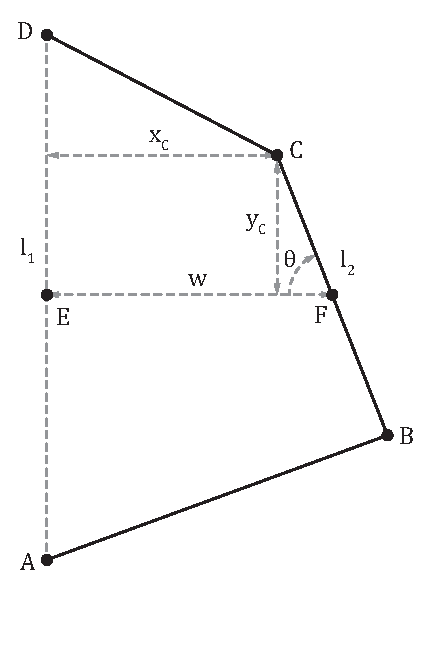
\includegraphics[width=3in]{figures/quad.eps}
  \caption{Minimizing perimeter around a quadrilateral}
\end{figure}

\subsection{Symmetric Quadrilateral}

Let us begin by solving the simplest version of this problem. Let us imagine that $s_b$ is connected to the midpoints of $s_1$ and $s_2$. We know that the perimeter will be given by $l_1 + l_2 + l_3 + l_4$ where $l_3$ and $l_4$ are the lengths of the sides of $s_3$ and $s_4$, respectively. We are given $l_1$ and $l_2$, but we will need to compute $l_3$ and $l_4$ as functions of $l_1, l_2,d, $ and $\theta$. 

We can find $l_3$ by using the fact that it forms a right triangle. We know that $l_3^2 = m^2 + n^2$. Finding $l_4$ is similar. Therefore, we just need to find $m$ and $n$. This can be done by using the fact that $m = \frac{l_1}{2} - \frac{l_2}{2} \sin \theta$. This is just the upper half of $s_1$ minus the projection of $s_2$ onto $s_1$. We can find $n$ similarly: $n = d - \frac{l_2}{2} \cos \theta$. This is just the bar $s_b$ minus the projection of $s_2$ onto the bar. Thus by substituting, we have:
\begin{eqnarray}
  l_3 = \sqrt{ \left(\frac{l_1}{2} - \frac{l_2}{2} \sin \theta \right)^2 + \left( d - \frac{l_2}{2} \cos \theta \right)^2 }
\end{eqnarray}

We can do a similar analysis on $l_4$, only remembering that $n$ for $l_4$ gets extended by the projection onto $s_4$ instead of shrunken. We therefore have:
\begin{eqnarray}
  l_4 = \sqrt{ \left(\frac{l_1}{2} - \frac{l_2}{2} \sin \theta \right)^2 + \left( d + \frac{l_2}{2} \cos \theta \right)^2 }
\end{eqnarray}

Now, to minimize the perimeter with respect to $\theta$, we want to minimize $l_1 + l_2 + l_3 + l_4$. Since we know that $l_1$ and $l_2$ are fixed, we really want to minimize $l_3 + l_4$ with respect to $\theta$. The other thing to note is that we're minimizing positive distances. We will invoke the following lemma so that we can simplify our expression for $\min l_3 + l_4$:

\begin{lemma}
  If $f(t), g(t) > 0$ and $k(t) > 0$ is a strictly monotonically increasing function for all $t$, then $\argmin_t k(f(t)) + k(g(t)) = \argmin_t f(t) + g(t)$.
  \label{lemma:minsqrt}
\end{lemma}
\proof Let $t_1, t_2$ be such that $f(t_1) + g(t_1) < f(t_2) + g(t_2)$. In this proof, we will show that $k(f(t_1)) + k(g(t_1)) < \sqrt{f(t_2)} + \sqrt{g(t_2)}$. Since $k(t)$ is a strictly monotonically increasing function when $t > 0$, we know that $k(x) < k(y)$ if and only if $x < y$ (assuming we can confine $x, y$ to be non-negative).

Because this is the case, we see that $k(f(x)) < k(f(y))$ if and only if $f(x) < f(y)$ (the same goes for $g$). Thus, we see that if we have found the minimum $t_m$ to $\argmin_t k(f(t)) + k(g(t))$, then it is the case that $k(f(t_m)) + k(g(t_m)) < k(f(t)) + k(g(t))$ for all $t \neq t_m$ (again where $t > 0$). Following our train of logic, we see that $f(t_m) + g(t_m) < f(t) + g(t)$ for all $t \neq t_m$, which means that $t_m$ is a minimum of $f(t) + g(t)$. Thus by finding a minimum $t_m$ to $k(f(t)) + k(g(t))$, we also found a minimum to $f(t) + g(t)$. \qed

Since we've proven this lemma, we can invoke it upon $\min l_3 + l_4$. Since $l_3 = \sqrt{z_3}$ and $l_4 = \sqrt{z_4}$, we can use $k(t) = \sqrt{t}$ and we can write $\min l_3 + l_4 = \min z_3 + z_4$ by using our lemma. Thus, we now want to solve the problem:
\begin{eqnarray}
  \argmin_{\theta} &2& \left(\frac{l_1}{2} - \frac{l_2}{2} \sin \theta \right)^2 \\
  &+& \left( d - \frac{l_2}{2} \cos \theta \right)^2 + \left( d + \frac{l_2}{2} \cos \theta \right)^2
\end{eqnarray}

Now, we can expand out our expression and use the fact that $\sin^2 \theta + \cos^2 \theta = 1$ to obtain a much simpler (but equivalent) minimization problem:
\begin{eqnarray}
  \argmin_{\theta} \frac{l_1^2}{2} + \frac{l_2^2}{2} + 2d^2 - l_1 l_2 \sin \theta
\end{eqnarray}

We note that $l_1, l_2,$ and $d$ are all constants which are given to us in the problem. Therefore, the minimization problem really boils down to
\begin{eqnarray}
  \argmin_{\theta} - l_1 l_2 \sin \theta = \argmax_{\theta} \sin \theta
\end{eqnarray}

Thus, we see that $\theta = \frac{\pi}{2}$ minimizes the perimeter of the quadrilateral in the symmetric case.

\subsection{Non-Symmetric Quadrilateral}

\section{Appendix}

\subsection{Notation\label{sec:notation}} 

\begin{description}
    \item[$t$] Time
    \item[$l$] Path length
    \item[$s$] Speed
    \item[$a_t$] Tangential acceleration
    \item[$a_c$] Centripetal acceleration
    \item[$\vec{x}$] Position
    \item[$\vec{v}$] Velocity
    \item[$\vec{a}$] Acceleration
\end{description}

\section{Coordinates}

\subsection{Scalar Calculus}

\begin{align}
s& = \frac{dl}{dt}\\
%
a_t& = \frac{ds}{dt}\\
\end{align}

\subsection{Vector Calculus}

\begin{align}
\boldsymbol{x}& = r \boldsymbol{\hat{r}}\\
%
\boldsymbol{\vec{v}}& = \dot{r} \boldsymbol{\hat{r}} + r \dot{\phi} \boldsymbol{\hat{\phi}}\\
%
\boldsymbol{\vec{a}}& = \paren{\ddot{r} - r \dot{\phi}^2} \boldsymbol{\hat{r}} + \frac{1}{r} \frac{d}{dt} \paren{r^2 \dot{\phi}} \boldsymbol{\hat{\phi}}
\end{align}

\subsection{Relations}

\begin{align}
l& = \int_{t=0}^{T} \norm{\boldsymbol{\vec{v}} \, } \; dt\\
%
s& = \boldsymbol{\vec{v}}\\
%
a_t& = \norm{\boldsymbol{\vec{a}}\,} \frac{\boldsymbol{\vec{v}}}{\norm{\boldsymbol{\vec{v}}\,}}
\end{align}

\bibliographystyle{plain}
\begin{thebibliography}{9}
\bibitem{wiki_pcoords}
\url{http://en.wikipedia.org/wiki/Polar_coordinate_system}
\end{thebibliography}

\end{document}

From Spring 2011 or before; revised by Miller, Spring 2013. 
